\documentclass[11pt]{article} 

\usepackage[utf8]{inputenc} 

\usepackage{geometry}
\geometry{a4paper}

\usepackage{graphicx}

%%% PACKAGES
\usepackage{float}
\usepackage{booktabs} % for much better looking tables
\usepackage{array} % for better arrays (eg matrices) in maths
\usepackage{paralist} % very flexible & customisable lists (eg. enumerate/itemize, etc.)
\usepackage{verbatim} % adds environment for commenting out blocks of text & for better verbatim
\usepackage{subfig} % make it possible to include more than one captioned figure/table in a single float
\usepackage{listings}
\usepackage{amsmath}
\usepackage{tikz}

\usetikzlibrary{positioning}


%%% HEADERS & FOOTERS
\usepackage{fancyhdr} % 
\pagestyle{plain} % options: empty , plain , fancy
\renewcommand{\headrulewidth}{0pt} % customise the layout...
\lhead{}\chead{}\rhead{}
\lfoot{}\cfoot{\thepage}\rfoot{}

%%% SECTION TITLE APPEARANCE
\usepackage{sectsty}
\allsectionsfont{\sffamily\mdseries\upshape} % (See the fntguide.pdf for font help)
% (This matches ConTeXt defaults)

%%% ToC (table of contents) APPEARANCE
\usepackage[nottoc,notlof,notlot]{tocbibind} % Put the bibliography in the ToC
\usepackage[titles,subfigure]{tocloft} % Alter the style of the Table of Contents
\renewcommand{\cftsecfont}{\rmfamily\mdseries\upshape}
\renewcommand{\cftsecpagefont}{\rmfamily\mdseries\upshape} % No bold!

%%% END Article customizations

%%% The "real" document content comes below...

\title{Statistical Machine Learning - Assignment 1}
\author{Joost Besseling and Luuk Verkleij}
%\date{}

\begin{document}
\lstset{language=Python}
\maketitle

\section{Introduction}
In this report, we will give an overview of the results that we obtained by implementing the various exercises of the assignment. In each section we will explain what we did, and why we did it in this way. 

As a short aside, we decided to write the code for this assignment in the Python programming language. This was purely out of practical reasons, since we both had no prior experience in Matlab. 

We used the Python library Matplotlib %Linkje naar matplotlib voor compleetheid van het 'selfcontained document'?
to create the graphs and other pictures in this document. We used the Numpy library as a replacement for all Matlab standard functions such as the \textbackslash - operator.

\section{Exercise 1}
For this exercise we are asked to consider the $M$-th order polynomial 
\[
y(x;\textbf{w}) = \sum^M_{j=0} w_j x^j
\]

and use it to approximate the following function:

\[
	f(x) = 1+ \sin(6(x-2)).
\]

We will lay-out what we did on a question by question basis. 

%1.1
\subsection{Noise}
\label{sec:noise}
In figure \ref{fig:noise} you can see the function $f$, as well as the $10$ observations that we made. This is the main training set, called $D_{10}$. The observations has Gaussian noise with a mean of zero and a deviation of 0.3. 
\begin{figure}[H]
	\centering
		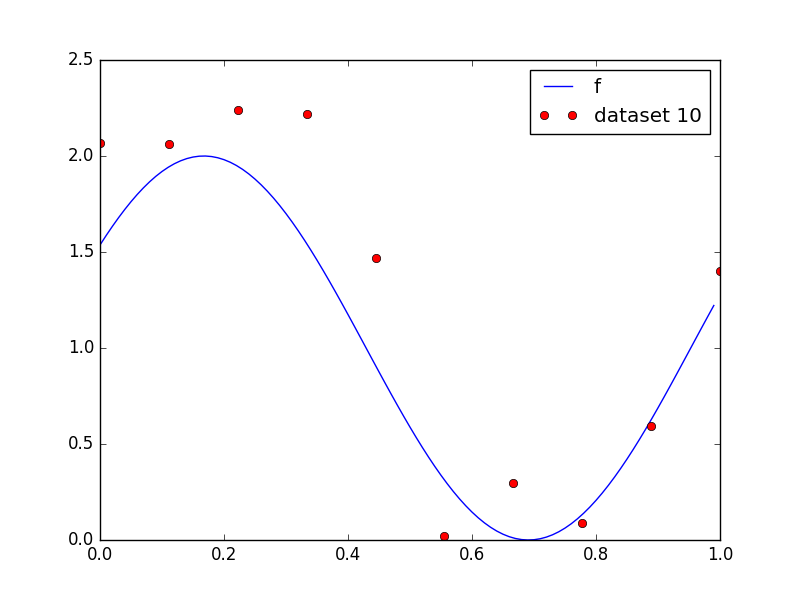
\includegraphics[trim={1cm 1cm 0.5cm 0.7cm},clip, scale=0.5]{images/exercise1_1.png}
		\caption{Function $f$ plotted and dataset $D_{10}$ with gaussian noise}
	\label{fig:noise}
\end{figure}

%1.2
\subsection{$PolCurFit$}
After creating the data points, we are asked to create a function that will fit a polynomial, in order to represent the original function.

Consider the polynomial $y(x;\textbf{w})$ and the error function 
\[
E(\textbf{w})= \frac{1}{2} \sum^N_{n=1} \left[y(x_n;\textbf{w})-t_n\right]^2
\]
where $x_n,t_n$ are the input/output pairs from the data set. Define the error per point as 
\[
E_n(\textbf{w})= \frac{1}{2} \left[y(x_n;\textbf{w})-t_n\right]^2,
\] note that $E = \sum^N_{n=1}E_n$. As in the exercises \cite{test}.

In order to fit the polynomial to the data points, we want to minimize the error function. In order to find the minimum, we find the gradient of the error function and set it equal to zero. First we find the gradient of $E$, $\nabla E$. Observe that $\nabla E = \sum^N_{n=1}\nabla E_n$. So it suffices to find the gradient of $E_n$ for $n\leq N$.
\[
\nabla E_n = \left(\frac{\partial E_n}{\partial w_0},\dots,\frac{\partial E_n}{\partial w_N}\right)
\]

We have 

\begin{align*}
\frac{\partial E_n}{\partial w_i} &= \frac{\partial }{\partial w_i} \cdot \frac{1}{2} \left[y(x_n;\textbf{w})-t_n\right]^2 \\
&= 2\cdot \left( \frac{1}{2} \left[y(x_n;\textbf{w})-t_n\right] \right) \cdot \frac{\partial  y(x_n;\textbf{w})}{\partial w_i} \\
\end{align*}
The right part evaluates to $x_n^i$, because $w_i$ is the $i$-th parameter of the polynomial. And the first part can be simplified to obtain the result

\[
\frac{\partial E_n}{\partial w_i} = \sum^M_{j=0}w_j x_n^{i+j} - t_n x_n^i
\]

So from $\nabla E = \sum^N_{n=1} \nabla E_n$, we find 
\[
\frac{\partial E}{\partial w_i} =\sum^N_{n=1}\left(\sum^M_{j=0}w_j x_n^{i+j} - t_n x_n^i\right).
\]

We are now ready to fine the following matrices:
\begin{align*}
A_{ij} &= \sum^N_{n=1} x_n^{i+j} \\
T_{i} &= \sum^N_{n=1}t_n x_n^i
\end{align*}

Now we obtain the following equation:
\begin{align*}
\frac{\partial E}{\partial w_i} &=\sum^N_{n=1}\left(\sum^M_{j=0}w_j x_n^{i+j} - t_n x_n^i\right) \\
&= \sum^M_{j=1}\sum^N_{n=0}w_j x_n^{i+j} - \sum^N_{n=1}t_n x_n^i  \tag{by applying simple transformations to the sum} \\
&=\sum^M_{j=0}A_{ij}w_j - T_i
\end{align*}
Since we want to minimize $E$, we try to find $\nabla E = 0$, so we find the following equation:

\begin{equation}
\label{eq:1}
\sum^M_{j=0}A_{ij}w_j-T_i = 0 \Rightarrow \sum^M_{j=0} A_{ij}w_j = T_i
\end{equation}

From this it follows that we can solve the equation for $\textbf{w}$ to find the polynomial with the smallest error function.

 We implemented the function PolCurFit as denoted in listing \ref{c:polcurfit2}.

\begin{lstlisting}[caption={PolCurFit}, label={c:polcurfit}]
def PolCurFit(x, t, m):
    # Exercise 2
    # D_n = (x, t)
    A = np.fromfunction(
        lambda i, j: sumx(x, i + j), (m + 1, m + 1), dtype=int)
    T = np.fromfunction(lambda i, j: sumy(x, t, i), (m + 1, 1), dtype=int)
    return np.linalg.solve(A, T)
\end{lstlisting}

In this listing, both $A$ and $T$ are numpy matrices that create matrices as we defined them earlier. \texttt{np.linalg.solve(A,T)} is the function that solves (\ref{eq:1}).
%1.3
\subsection{Plotting $PolCurFit$ trained on $D_{10}$}
\label{sec:d10}
Using the dataset with noise $D_{10}$ we generate polynomials of order 0 through 9 using $PolCurFit$. We are plotting the resulting polynomials and for each polynomial we compute the root-mean-square error for both training set $D_{10}$ and test set $T$.

\subsubsection{$D_{10}$ Training Set}
\label{sec:d10plots}
In figure \ref{fig:d10plots} the training set $D_{10}$ is plotted together with the polynomial functions generated by the $PolCurFit$. We see that the polynomial functions with higher order are fitting better, until around order 7, where overfitting starts to occur. The  polynomial function with order 9 goes through all the points of $D_{10}$, but it does not match $f$ very well.

\begin{figure}[H]
	
	\centering
		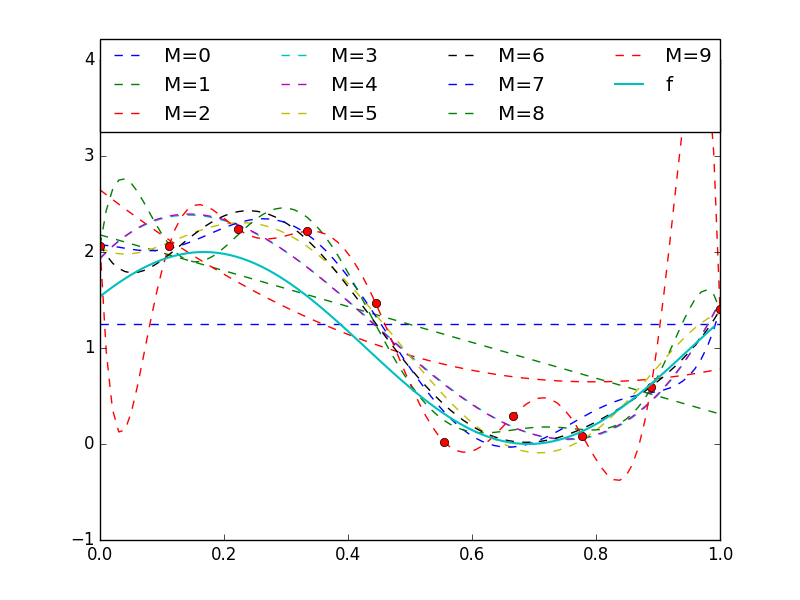
\includegraphics[trim={1cm 1cm 0.5cm 0.7cm},clip, scale=0.5]{images/exercise1_3a.png}
		\caption{Polynomial functions from $PolCurFit$, based on training set $D_{10}$, with order 0 through 9. }
	\label{fig:d10plots}
	
\end{figure}

\subsubsection{root-mean-square error}
\label{sec:d10error}
To find out which polynomial fits the best and which polynomial is an overfit, we can calculate the root-mean-square error or the $E_{RMS}$. The $E_{RMS}$ is calculated as follows:
\[
E_{RMS} = \sqrt{2E(\mathbf{w*})/N} = \sqrt{\frac{1}{N} \sum^N_{n=1} \left[y(x_n;\textbf{w*})-t_n\right]^2}
\]

We calculate the $E_{RMS}$ both for the training set $D_{10}$ and for the test set $T$. Test set $T$ is a set of 100 observations with Gaussian noise, like $D_{10}$, where the mean is 0 and the deviation is 0.3.

In figure \ref{fig:d10error} the $E_{RMS}$ is plotted. What we find is that overfitting starts occurring around order 5, where the root-mean-square error with the test set is getting larger compared to the previous polynomial. What we also find is that the $E_{RMS}$ for the test set is getting smaller, to eventually zero. This is as expected, as the polynomial function of order 9 goes through every point, as we can see in figure \ref{fig:d10plots}. Note that the image is not the same as in Bishop, we even see that the test set is a better fit for the first 3 values. This is because the distribution of the datapoints was rather unlucky. We noticed that changing the random-seed gave us wildly varying results, but we decided to stick to the first seed that we used (which is $0$).


\begin{figure}[H]
\centering
	\begin{tikzpicture}
	\node(d10error){	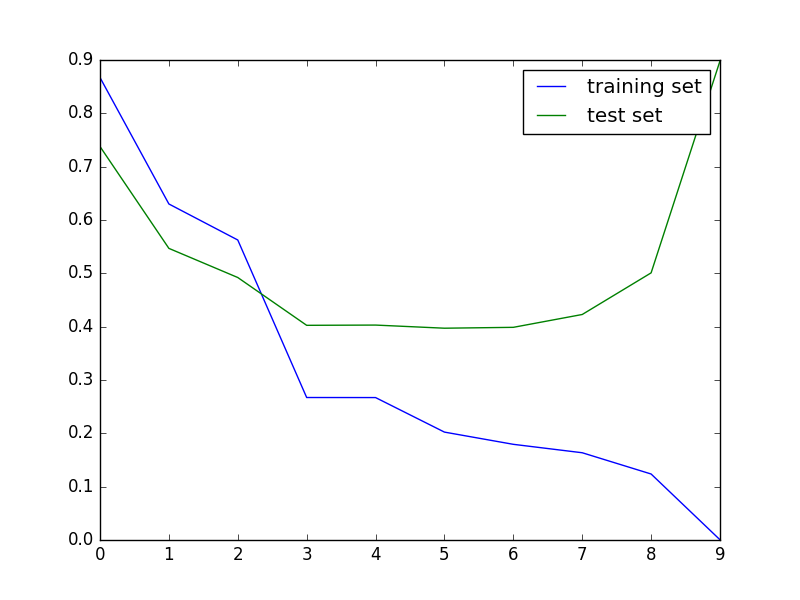
\includegraphics[trim={1cm 1cm 0.5cm 0.7cm},clip, scale=0.5]{images/exercise1_3b.png}};
	\node[below=of d10error, node distance=0cm, yshift=1cm,font=\color{black}] {Order};
	\node[left=of d10error, node distance=0cm, rotate=90, anchor=center,yshift=-0.7cm,font=\color{black}] {$E_{RMS}$};
	\end{tikzpicture}
	\centering
	\caption{Plot of the $E_{RMS}$ for both $D_{10}$ and $T$, compared to the polynomial functions plotted in figure \ref{fig:d10plots}}
	\label{fig:d10error}

\end{figure}

%1.4
\subsection{Plotting $PolCurFit$ trained with $D_{40}$}
Similar to section \ref{sec:d10} we generate polynomials for order 0 through 9 using $PolCurFit$, but this time with dataset $D_{40}$. We are plotting the resulting polynomials and for each polynomial we compute the root-mean-square error for both training set $D_{40}$ and test set $T$. 
 Like $D_{10}$, $D_{40}$ is a dataset with 40 observations, uniformly spaced with Gaussian noise.

\subsubsection{$D_{40}$ Training Set}
We do the same as section \ref{sec:d10plots}, but with $D_{40}$. What we find is that there is no obvious over fitting, and we find that the polynomial functions are a better fit. This is because with $4$ times as many data points, it is impossible for the polynomial of order 9 to fit all points. So the function 'tries' to fit the function. The chance that a lot of the observations are, for example, located above the function, as we see with our $D_{10}$ data set, also becomes lower. So we expect that the $E_{RMS}$ of the training set and the test set are a lot closer to each other.

\begin{figure}[H]
	\centering
		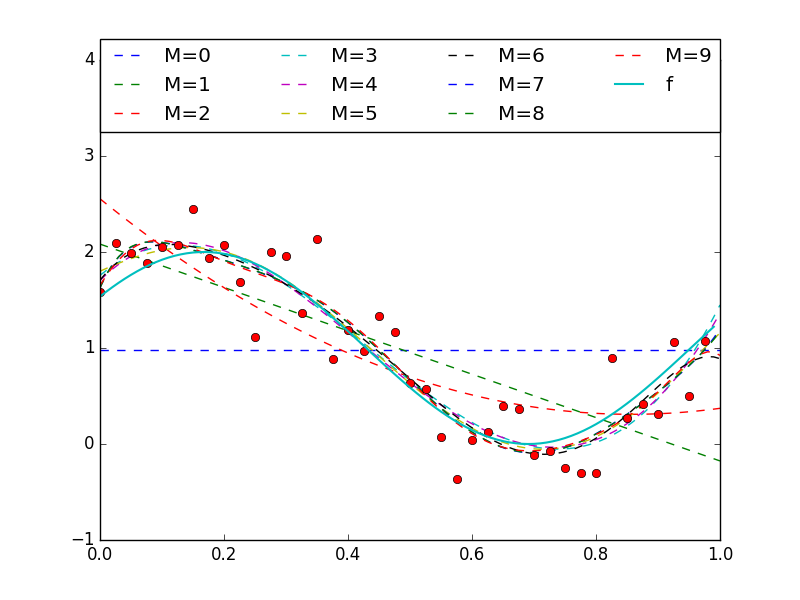
\includegraphics[trim={1cm 1cm 0.5cm 0.7cm},clip, scale=0.5]{images/exercise1_4a.png}
		\caption{Polynomial functions from $PolCurFit$, based on training set $D_{40}$, with order 0 through 9. }
	\label{fig:d40plots}
\end{figure}

\subsubsection{root-mean-square error}
We do the same as section \ref{sec:d10error}, but with training set $D_{40}$. As we observed with figure \ref{fig:d40plots}, we find that $E_{RMS}$ is a lot lower in figure \ref{fig:d40error}. Again, this is because with more data, the average of the data is closer to the real function. We find that a possible solution for over fitting is a higher number of observations.

\begin{figure}[H]
	\begin{tikzpicture}
	\node(d40error){	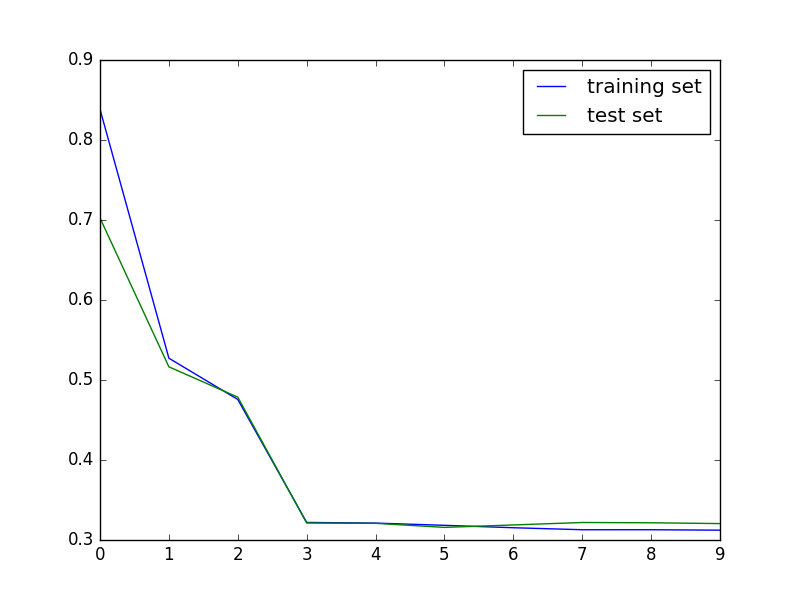
\includegraphics[trim={1cm 1cm 0.5cm 0.7cm},clip, scale=0.5]{images/exercise1_4b.png}};
	\node[below=of d40error, node distance=0cm, yshift=1cm,font=\color{black}] {Order};
	\node[left=of d40error, node distance=0cm, rotate=90, anchor=center,yshift=-0.7cm,font=\color{black}] {$E_{RMS}$};
\end{tikzpicture}
\centering
	\centering
		
		\caption{Plot of the $E_{RMS}$ for both $D_{40}$ and $T$, compared to the polynomial functions plotted in figure \ref{fig:d10plots}}
	\label{fig:d40error}
\end{figure}

%1.5
\subsection{$PolCurFit$ with an additional penalty parameter $\lambda$}

Now we change $PolCurFit$ to avoid the over fitting problem that we have seen in section \ref{sec:d10} with the data set $D_{10}$.

We let 
\[
	\tilde{E} = E + \frac{\lambda}{2} \sum_{j=0}^{M} w_j^2.
\]
We show that this does not change much in the way we obtain the value of $\textbf{w}$.
 Since 
 
\begin{align*}
  \frac{\partial\tilde{E}}{\partial w_i} &= \frac{\partial E}{\partial w_i} + \frac{\partial}{\partial w_i}(\frac{\lambda}{2} \sum_{j=0}^{M} w_j^2) \\
  &= \frac{\partial E}{\partial w_i} + \lambda w_i. \\  
\end{align*}
We can simplify this, by incorporating the $\lambda$ parameter into $A$ as follow:
$\tilde{A}_{ij} = A_{ij} + \lambda\delta_{ij}$.
So in order to do this, all we have to change is the generation of the $A$-matrix in our code: Using this we have changed the $PolCurFit$ function. The new code can be found in listing \ref{c:polcurfit2}.

\begin{lstlisting}[caption=$PolCurFit2$, label=c:polcurfit2]
def PolCurFit2(x, t, m, lbd):
    # Exercise 5
    # Sum_j=0^M Aij * wj = Tj
    # Based on exercise sheet 2, exercise 2.3
    A = np.fromfunction(
    lambda i, j: sumx(x, i + j) + lbd * kdelta(i, j),
        (m + 1, m + 1),
        dtype=int)
    T = np.fromfunction(lambda i, j: sumy(x, t, i), (m + 1, 1), dtype=int)
    return np.linalg.solve(A, T)
\end{lstlisting}

Using $PolCurFit2$ we have plotted the new polynomials using the $D_{10}$ and $\ln\lambda = -18$ in fig \ref{fig:lambdaplot}. Here we do not see the over fitting of the polynomial with order 9, while using the same dataset. 

\begin{figure}[H]
\centering
	\centering
		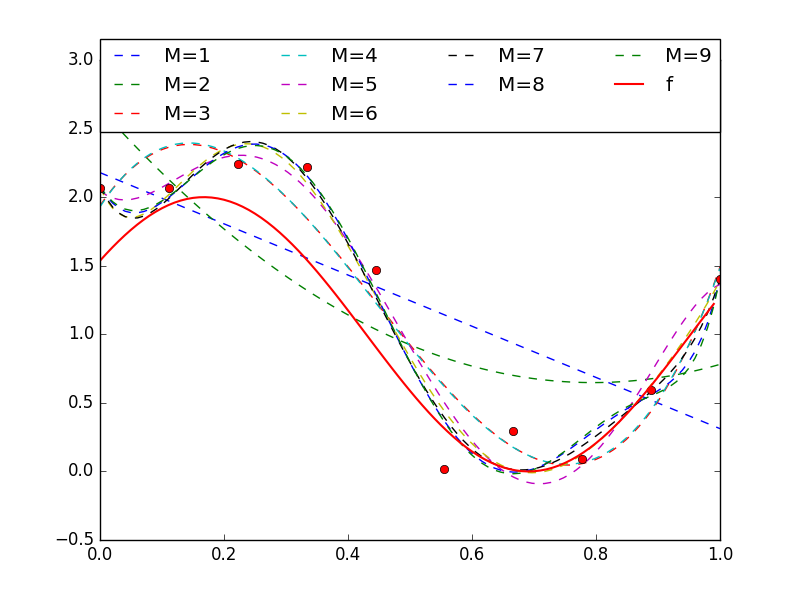
\includegraphics[trim={1cm 1cm 0.5cm 0.7cm},clip, scale=0.5]{images/exercise1_5.png}
		\caption{plots of polynomials generated by $PolCurFit$, with $\ln\lambda = -18$} 
	\label{fig:lambdaplot}
\end{figure}

Using the $E_{RMS}$ we can see the impact of the regularization term. We plotted both the $E_{RMS}$ for the training set as the data set against $\ln\lambda$ in figure \ref{fig:lambdaerror}. We see that the $\lambda$ term now controls the size of $|\textbf{w}|$ and therefore the overfitting, since the $\lambda$ term drives down all co\"efficient of the higher order polynomials.

\begin{figure}[H]
\centering
	\centering
		\begin{tikzpicture}
			\node(lambdaerror){	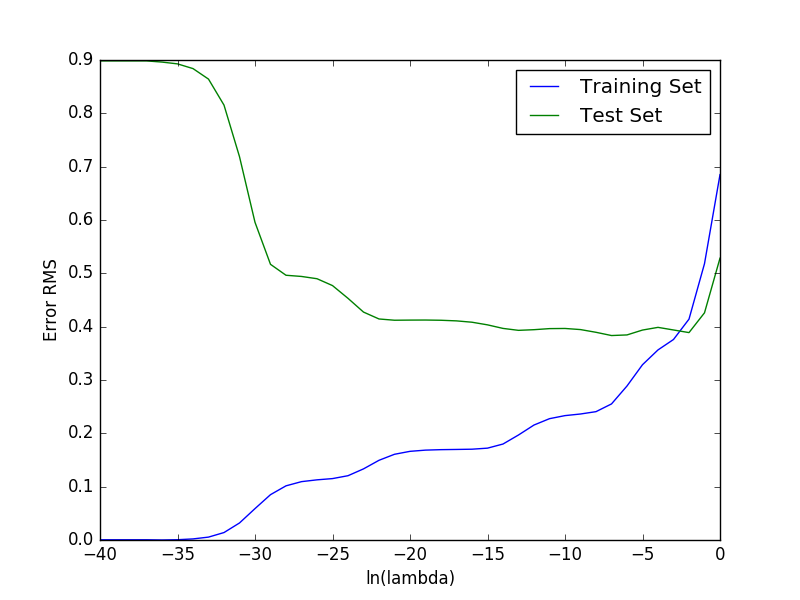
\includegraphics[trim={1.5cm 1cm 0.7cm 0.7cm},clip, scale=0.5]{images/exercise1_5_1.png}};
			\node[below=of lambdaerror, node distance=0cm, yshift=1cm,font=\color{black}] {$\ln\lambda$};
			\node[left=of lambdaerror, node distance=0cm, rotate=90, anchor=center,yshift=-0.7cm,font=\color{black}] {$E_{RMS}$};
		\end{tikzpicture}		
		\caption{Plot of $E_{RMS}$ of polynomial with order 9 with variant $\lambda$ term. This figure is comparable by Bischop figure 1.8} 
	\label{fig:lambdaerror}
\end{figure}

We can see that the regularizer drives the weights of high order terms towards zero in figure \ref{fig:highorder}

\begin{figure}[H]
	\centering
		\centering
		\begin{tikzpicture}
			\node(highorder){	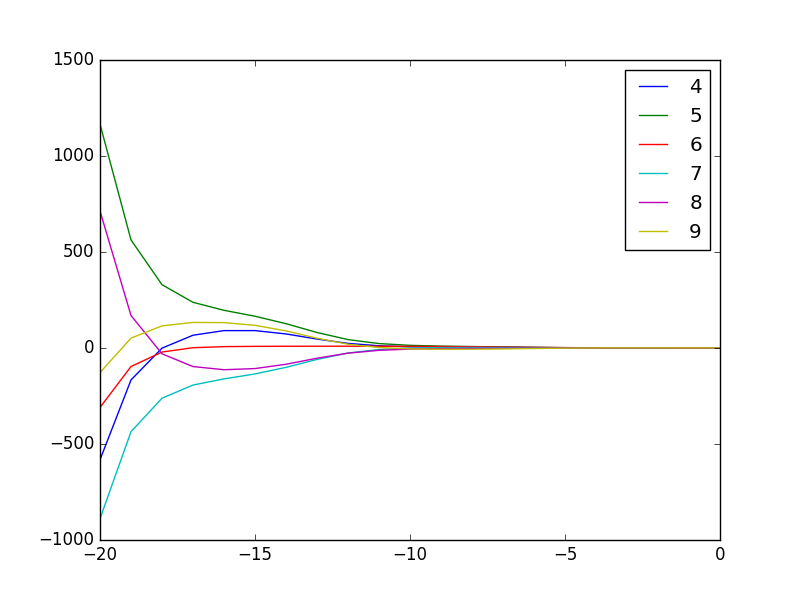
\includegraphics[trim={1cm 0cm 0.5cm 0.7cm},clip, scale=0.5]{images/exercise1_5_2.png}};
			\node[below=of highorder, node distance=0cm, yshift=1cm,font=\color{black}] {$\ln\lambda$};
			\node[left=of highorder, node distance=0cm, rotate=90, anchor=center,yshift=-0.7cm,font=\color{black}] {$coefficent$};
		\end{tikzpicture}	
		\caption{Plot of the terms, where 9 is the coefficent of the term $x^9$, etc.} 
	\label{fig:highorder}
\end{figure}

\section{Exercise 2}
In this exercise we are looking at the function $h(x,y)$ and at gradient descent iteration. $h(x,y)$ is defined as:
\[
h(x,y) = 100(y - x^2)^2 + (1 - x)^2
\]

and a gradient descent iteration step is defined as:
\[
w_{n+1} = w_n - \eta \nabla E(w_n)
\]

where $w_n$ is a vector and $\nabla E(w_n)$ is the gradient of a function. The $\eta$ is  step size, and if $\eta$ is small enough it will converge. 


\subsection{Surface plot of $h(x,y)$}
We have plotted $h(x,y)$ as shown in figure \ref{fig:surface}. As we can see the gradient is  big on the slopes of $h$, and small in the valley of $h(x,y)$. This means that we need low $\eta$ for our gradient descent, otherwise the algorithm will jump from one side of the valley to the other, without getting closer to the minimum. But because the gradient is small in the valley of $h$, it will take a long time to get to the minimum once it is in the valley. As a result the gradient descent will be slow.

\begin{figure}[H]
	\centering
		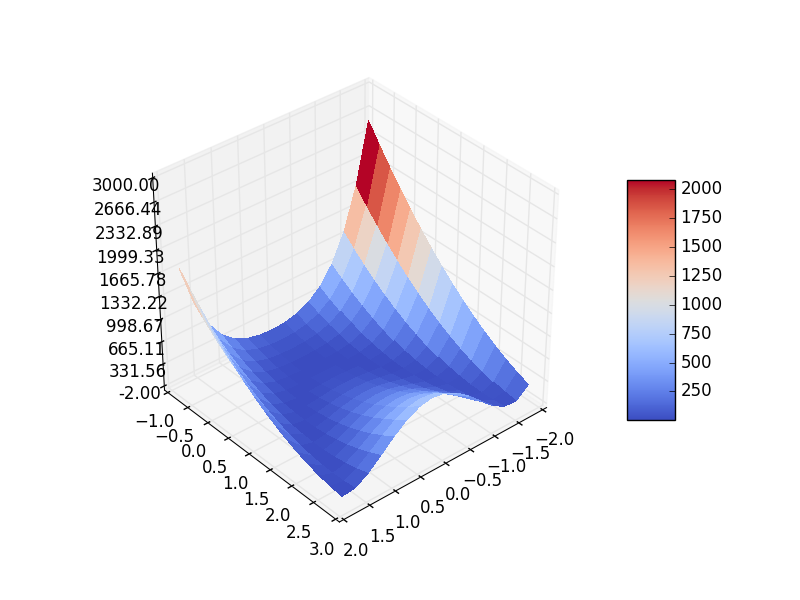
\includegraphics[trim={1cm 1cm 0.5cm 0.7cm},clip, scale=0.7]{images/exercise2_1.png}
		\caption{The surface plot of $h(x,y)$}
	\label{fig:surface}
\end{figure}

\subsection{}

Here we show that $(1,1)$ is the unique minimum of $h(x, y)$.
$h(x, y)$ is minimum when $\nabla h(x,y) = (0,0)$.

\begin{align*}
\nabla h(x,y) & = (2 (200 x^3-200 x y+x-1), 200 (y-x^2)) \\
& \Rightarrow 200y - 200x^2 = 0 \\
& \Rightarrow y = x^2
\end{align*}

Substitute $y = x^2$

\begin{align*}
0 & = (2(200x^3 - 200x(x^2) + x - 1)) \\
0 & = 2(0 + x - 1) \\
0 & = 2x - 2 \\
x &= 1
\end{align*}

Therefore the only solution for $x$ is $1$. Substitute $x = 1$ to find $y$.

\begin{align*}
0 & = 200(y - (1)^2) \\
0 & = 200y - 200 \\
y & = 1
\end{align*}

Therefore the only solution for $y$ is $1$, assuming $x=1$, which is unique. Therefore the unique minimum for $h(x,y)$ is $(1,1)$.
\subsection{The Descent Iteration Rule}
The descent iteration rule is 
\[
	w_{n+1} = w_n - \eta \nabla E(w_n)
\]

To find our iteration rule we take $\nabla E(w_n)$ is $\nabla h(x,y) = (2 (200 x^3-200 x y+x-1), 200 (y-x^2))$. Therefore our iteration rule is as follows:
\[
w_{n+1} = w_n - \eta \nabla h(w_n)
\]

And filled in the descent iteration rule for $h(x,y)$ is as follows:

\[
(x_{n+1},y_{n+1}) = (x_n,y_n) - \eta (400 x^3-400 x y+2x-2, 200y-200x^2)
\]

\subsection{Gradient Descent}

We have implemented and used the gradient descent iteration. Using different steps of $\eta$ we found that it needs to be low for the gradient decent iteration to converge. In table \ref{tbl:eta} we find that that the lowest $\eta$  that converges from all the three starting points is 0.001, with an average of around 50000 steps. 

\begin{table}[H]
	\centering
	\label{tbl:eta}
	\begin{tabular}{|l|l|l|l|l|}
		\hline
		\textbf{Starting Point} & \textbf{$\eta$ = 0.01} & \textbf{$\eta$ = 0.0015} & \textbf{$\eta$ = 0.001} & \textbf{$\eta$ = 0.0001} \\ \cline{2-5} 
		\textbf{(-2, -1)}       & diverges               & diverges                 & 49273                   & 487202                   \\ \cline{2-5} 
		\textbf{(0, 3)}         & diverges               & 32347                    & 48477                   & 482023                   \\ \cline{2-5} 
		\textbf{(-2, 3)}        & diverges               & 33036                    & 51912                   & 544560                   \\ \hline
	\end{tabular}
	\caption{The steps required for the gradient descent iteration to diverge}
\end{table}

We have also plotted the trajectory for the three different starting points in figure \ref{fig:eta0015}, \ref{fig:eta001} and \ref{fig:eta0001}

\begin{figure}[H]
	\centering
		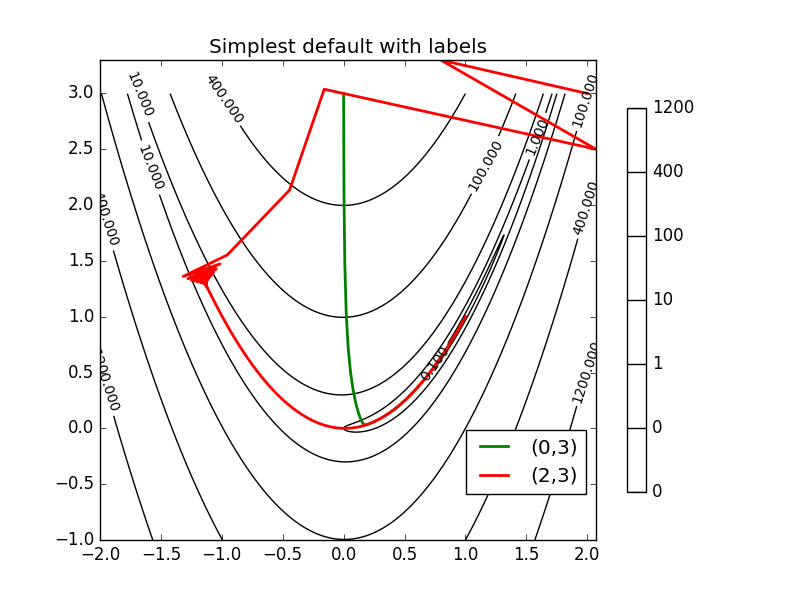
\includegraphics[trim={1cm 1cm 0.5cm 0.7cm},clip, scale=0.5]{images/exercise2_4_1.png}
		\caption{Trajectories with $\eta = 0.0015$}
	\label{fig:eta0015}
\end{figure}

\begin{figure}[H]
	\centering
	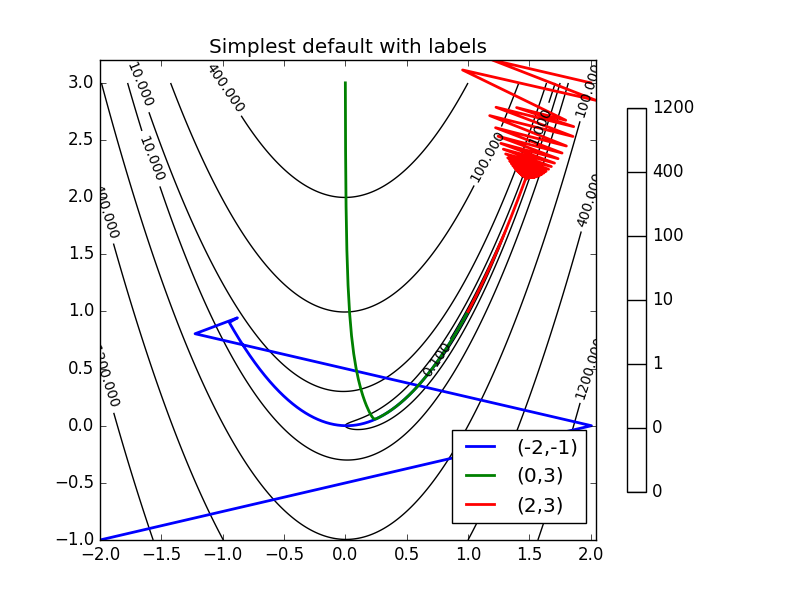
\includegraphics[trim={1cm 1cm 0.5cm 0.7cm},clip, scale=0.5]{images/exercise2_4_2.png}
	\caption{Trajectories with $\eta = 0.001$}
	\label{fig:eta001}
\end{figure}

\begin{figure}[H]
	\centering
	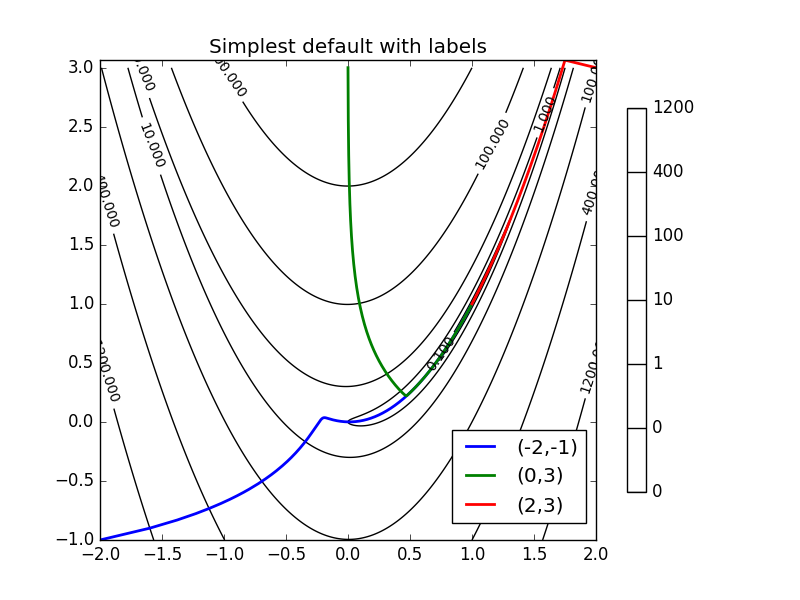
\includegraphics[trim={1cm 1cm 0.5cm 0.7cm},clip, scale=0.5]{images/exercise2_4_3.png}
	\caption{Trajectories with $\eta = 0.0001$}
	\label{fig:eta0001}
\end{figure}

What we find is that it is possible for a trajectory to bounce around the valley, where it goes from one steep slope, to another steep slope. This is very obvious from fig \ref{fig:eta0015}, where we can see this effect from starting point (2,3), even though it converges. To counter act this we need a low $\eta$ and therefore our gradient descent iteration is slow, as we mentioned in the introduction of this section.

\section{Exercise 3}

After all this hard work, it is time for a healthy snack. But first, we have to pick a fruit. Curiously enough, we have two boxes standing before us, one box is filled with $8$ apples and $4$ grapefruits, the other box contains $15$ apples and $3$ grapefruits. To decide which fruit we get, we first randomly pick a box, and after that we pick a first piece. We put it back, and from the same box we pixk a second piece randomly.

For simplicity, we call the box with 4 grapefruits the small box, and the box with 15 apple the big box.

\subsection{$P(F_1=apple|F_2=grapefruit)$}
From the fact that the second piece was a grapefruit, we can deduce that there is a higher chance that we are picking our fruit from the big box. But it does of course not affect the chance that we pick either an apple or a grapefruit from that specific box.

So we calculate the chance that we pick the small box, given that we picked a grapefruit. Obviously, the chance that we pick the small box is $1/2$, and the unconditional chance that we pick a grapefruit is easily calculated and is $17/30$.
\begin{align*}
P&(B=small|F_2=grapefruit)  \\
 &= P(F_2=grapefruit|B=small)\cdot\frac{P(B=small)}{P(F_2=grapefruit)}    \tag{Bayes' rule}\\
&= \frac{4}{12}\cdot \frac{1}{2}\big/\frac{17}{30} = 5/17
\end{align*}

From this we can calculate the chance that we picked an apple:
\begin{align*}
P(F_1=apple|F_2=grapefruit) &=  P(F_1=apple|B=small)\cdot P(B=small|F_2=grapefruit)\\ & \ \ \ + P(F_1=apple|B=big)\cdot P(B=big|F_2=grapefruit) \\
&=8/12\cdot 5/17 + 3/15\cdot 12/17.
\end{align*}

You might think: How can the result of the second pick affect the probability of the
first pick? But if we know that we got a grapefruit as the second fruit, we gain some knowledge about which box the fruit was picked from. It is clear that picking the fruit from a different box, gives a different chance for the fruit. So we also get some knowledge about the probability of the chance that we picked an apple.


\subsection{Oranges}
In this case, $P(F_2=grapefruit|B=small) = 1/6$ and $P(F_2=grapefruit|B=big) = 1/6$ as well. So it does not matter which box we pick from. This means that knowing that we picked a grapefruit, does not influence the probabilities of the second pick. This does not mean that the two picks are independent: Assume that the first pick was an orange. It is clear that the chance that we pick an orange again just got a lot bigger, since now we know that we are picking our fruits from the small box. 




\end{document}
